
\chapter{动态推荐系统设计}
  \section{前言}
  推荐系统的形式化定义如下:设C是所有用户的集合,S是所有可以推荐给用户的主题的集合。实际上,C和S集合的规模通常很大,如上百万的顾客以及上万款手机主题。设效用函数u()可以计算主题s对用户c的推荐度(如提供商的可靠性(vendor reliability)和产品的可得性(product availability)等),即$u=C\times S \rightarrow R$,R是一定范围内的全序的非负实数,推荐要研究的问题就是找到推荐度R最大的那些主题S*,如\autoref{equ:fromal}
    \begin{equation}
    \forall c \in C,S^{*}=arg  max_{s \in S} u(c,s)
    \label{equ:fromal}
    \end{equation}
  除了推荐系统自身如冷启动、数据的稀疏性等问题,还有一个关注点就是推荐系统的时间效应问题。比较常见的时间效应问题主要反映在用户兴趣的变化、物品流行度的变化以及商品的季节效应,这些问题都可以利用用户画像解决。本章节主要介绍如何搭建一个具有长尾性、实时性的动态推荐系统。动态推荐形态由3个重要的模块组成:用户画像模型,用户兴趣探索模块、推荐主题模块、推荐算法模块。通用的推荐系统模型流程如所示。推荐系统把用户画像模型中兴趣需求信息和推荐主题模型中的特征信息匹配,同时使用相应的推荐算法进行计算筛选,找到用户可能感兴趣的推荐主题,然后推荐给用户。

  用户画像模块对应着用户长期兴趣,用户兴趣探索对应着用户短期动态兴趣。短期兴趣的特点是临时、易变;长期兴趣的特点是长久、稳定;用户的短期兴趣可能会转化为长期兴趣,所以需要在推荐时综合考虑长期兴趣和短期兴趣。考虑到推荐系统的时间效应问题,将输入数据集归结为一个四元组,即{用户,物品,行为,时间},通过研究用户的历史行为来预测用户将来的行为。需要解决以下俩个问题:动态评分预测、时效性的影响。首先,动态评分预测问题。数据集可以选用比较直观的显性反馈数据集,即(用户,物品,评分,时间),研究是这样一个问题,给定用户u,物品i,时间t,预测用户u在时间t对物品i的评分r。对于该类问题,与时间无关的评分预测问题算法主要有以下几种:用户兴趣的变化,如年龄增长,从儿童长成青少年壮年;生活状态的变化,由以前的小学生到大学生;社会事件的影响如俩会等。此外还有季节效应问题,一些在春季很流行的,在夏季节未必就很流行。该问题的解决有待进一步思考。对于时效性的影响,每个在线系统都是一个动态系统,但它们有不同的演化速率。比如说,新闻,手机主题更新很快,但音乐,电影的系统演化的却比较慢。

  本章首先介绍用户画像和兴趣探索模块,其中兴趣探索模块需要根据业务的演化速率来调整迭代深度。然后介绍推荐主题模块,之后介绍推荐算法模块和指标体系,最后做总结。
  
  \section{用户画像和兴趣探索模块}
  目前基于用户画像的推荐,主要用在基于内容的推荐,从最近的RecSys大会(ACM Recommender Systems)上来看,不少公司和研究者也在尝试基于用户画像做Context-Aware的推荐(情境感知,又称上下文感知)。利用用户的画像,结合时间、天气等上下文信息,给用户做一些更加精准化的推荐是一个不错的方向。一个好的推荐系统要给用户提供个性化的、高效的、动态准确的推荐,那么推荐系统应能够获取反映用户多方面的、动态变化的兴趣偏好,推荐系统有必要为用户建立一个用户兴趣探索模型,该模型能获取、表示、存储和修改用户兴趣偏好,能进行推理,对用户进行分类和识别,帮助系统更好地理解用户特征和类别。推荐系统根据用户画像进行推荐,所以用户画像对推荐系统的质量有至关重要的影响。建立用户画像模型之前,需要考虑:模型的输入数据有哪些,如何获取模型的输入数据;如何考虑用户的兴趣及需求的变化;建模的对象是谁以及如何建模;模型的输出是什么。用户画像模型的输入数据主要有以下几种:
  \begin{itemize}
  \item 用户属性,分为社会属性和自然属性,包括用户最基本的如用户的姓名、年龄、职业、收入、学历等信息。用户注册时的对自然属性和社会属性进行初始建模。 
  \item 用户手工输入的信息:是用户主动输出给系统的信息,包括用户在搜索引擎中打出的关键词,用户评论中发布的感兴趣的主题、频道。还有一类重要的信息就是用户反馈的信息,包括用户自己对推荐结果的满意程度;用户标注的浏览页面的感兴趣、不感兴趣或感兴趣的程度等。
  \item 用户的浏览行为和浏览内容:用户浏览的行为和内容体现了用户的兴趣和需求,它们包括浏览次数、频率、停留时间等,浏览页面时的操作(收藏、保存、复制等)、浏览时用户表情的变化等。服务器端保存的日志也能较好地记录用户的浏览行为和内容。
  \item 推荐对象的属性特征:不同的推荐对象,用户建模的输入数据也不同。网页等推荐对象通常考虑对象的内容和用户之间的相似性,而产品等推荐对象通常考虑用户对产品的评价。为提高推荐质量,推荐对象的相关的属性也要考虑进去,比如除网页内容以外,还要考虑网页的发布人、时间等。产品类的对象还要考虑产品的品牌、价格、出售时间等。
  \end{itemize}

  用户行为的权重排序。用户显式行为数据记录了用户在平台上不同的环节的各种行为,这些行为一方面用于候选集触发算法中的离线计算(主要是点击、浏览),另外一方面,这些行为代表的用户兴趣强弱不同,因此在训练重排序模型时可以针对不同的行为设定不同的权重值,以更细地刻画用户的行为强弱程度。此外,用户的购买、试用等行为还可以作为重排序模型的交叉特征,用于模型的离线训练和在线预测。负反馈数据反映了当前的结果可能在某些方面不能满足用户的需求,因此在后续的候选集触发过程中需要考虑对特定的因素进行过滤或者降权,提高用户体验;同时在重排序的模型训练中,A/B测试结果可以作为不可多得的负例参与模型训练。用户画像是刻画用户属性的元数据,其中有些是直接获取的基础数据,有些是经过挖掘的二次数据,这些属性一方面可以用于候选集触发过程中对标签进行加权或降权,另外一方面可以作为重排序模型中的用户维度特征。通过对数据的挖掘可以提取出一些关键词,然后使用这些关键词给主题打标签,用于主题的个性化展示。

  用户行为的获取方式。模型输入数据的方式有显式获取、隐式获取和启发式获取三种方式。显式获取用户兴趣偏好的方法是简单而直接的做法,能准确地反映用户的需求,同时所得的信息比较具体、全面、客观,结果比较可靠。缺点就是数量稀少,原因用户不太愿意花时间来向商家表达自己的喜好,并且这种方法灵活性差,答案存在异质性,当用户兴趣主题改变时需要用户手动更改系统中用户兴趣。同时该方法对用户不是很人性化。解决人性化问题是推荐系统未来的一个研究方向,来研究用户能够接受的评价方式是什么,比如能够有耐心进行几次评分。利用固定负担模型来计量用户评价的负担,将人性化设计问题转化为最优化问题来研究。隐式获取法是指系统通过记录用户行为数据,通过权重排序获取用户的兴趣偏好,用户的很多动作都能暗示用户的喜好,包括查询、浏览页面和文章、标记书签、反馈信息、滑屏等。隐式的跟踪可以在建立用户画像基本数据的同时不打扰用户的正常消费活动。这种方法的缺点就是跟踪的结果未必能正确反映用户的兴趣偏好。同时系统若过度跟踪用户的历史记录,有时会引发用户隐私问题,而放弃对当前推荐系统的使用。 上述获取兴趣偏好的方法有时受用户教育背景、职业和习惯等因素的限制,用户有时意识不到自己的兴趣主题,因此能为用户提供启发式信息,如领域术语抽取和相似度物品聚类,可以实现领域知识的复用,为用户间的协同提供支持,提高用户兴趣获取质量。用户的兴趣和需求会随着时间和情景发生变化,用户画像模块要考虑到用户长期兴趣偏好和短期兴趣偏好,还要考虑兴趣的变化,目前很多研究关注了用户的长期兴趣,建立了静态用户画像模型,但用户兴趣探索模型也越来越受到关注。结合长期和短期兴趣的动态建模将是未来的一个研究方向,如\autoref{pic:hl_iterate}所示。
  \begin{figure}
    \centering
      \framebox{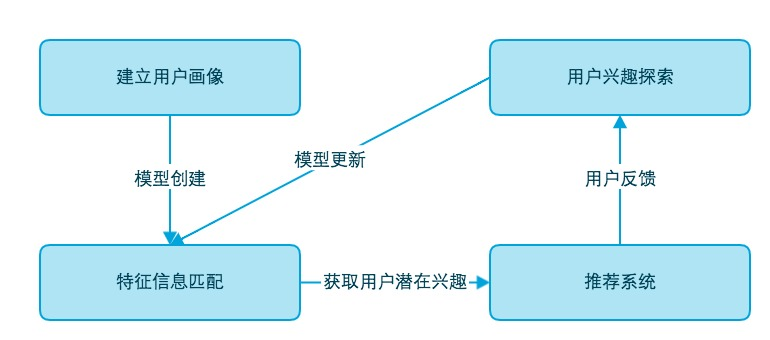
\includegraphics[scale=0.4]{figures/hl_iterate}}
      \figcaption{用户画像的使用}
      \label{pic:hl_iterate}
  \end{figure}

  用户画像更新采用了时间窗方法和遗忘机制来反映用户兴趣的变化。目前的更新机制无法及时跟踪用户兴趣的变化,just-in-time型有更强学习效率和动态变化适应能力的建模也是未来的重要研究方向。 

  \section{推荐主题模块}
  推荐主题分为单用户建模和群组建模,单用户建模针对个体用户进行建模,比如基于主题款式的推荐,群组建模是针对一类用户进行建模,比如基于商品的协同推荐。

  应用于不同的领域的推荐系统其推荐的商品特点也各不相同,如何对推荐主题进行描述对推荐系统也有很重要的影响。和用户画像一样,要对推荐主题进行描述之前要考虑:提取推荐主题的什么特征,如何提取,提取的特征用于什么目的,主题的特征描述和用户画像之间有关联。提取到的每个主题特征标签对推荐结果会有什么影响。主题的特征描述文件能否自动更新。
  推荐主题的描述文件中的主题特征和用户画像中的兴趣标签进行推荐计算,获得推荐主题的推荐权重,所以推荐主题的描述文件与用户画像密切相关,通常的做法是用同样的方法来表达用户的兴趣偏好和推荐主题。推荐系统推荐主题包括众多的领域,比如体育、动漫、科技还有诸如音乐、电影等多媒体资源等等。不同的主题,特征也不相同,目前并没有一个统一的标准来进行统一描述,主要有基于内容的方法和基于分类的方法两大类方法。 基于内容的方法是从主题本身抽取相关信息来表示主题,使用最广泛的方法是用加权关键词矢量,该方法通过对标注主题的标签进行统计分析得出的特征向量。方法很多,比较简单的做法就是计算每个特征的熵,选取具有最大熵值的若干个特征;也可以计算每个标签的信息增量(Information gain),即计算每个特征在主题中出现前后的信息熵之差;还可以计算每个特征的互信息(mutual information),即计算每个特征和主题的相关性。在完成主题特征提取后,还需要计算每个特征的权值,权值大的对推荐结果的影响就大。基于分类的方法是把推荐主题放入不同类别中,这样可以把同类主题推荐给对该类主题感兴趣的用户了。文本分类的方法有多种,比如朴素贝叶斯(Naive-Bayes),k最近邻方法(KNN)和支持向量机(SVM)等。 主题的类型可以预先定义,也可以利用聚类算法自动产生。研究表明聚类的精度非常依赖于主题的数量,而且由自动聚类产生的类型可能对用户来说是毫无意义的,因此可以有选择的进行手工选定的类型来分类主题,在没有对应的候选类型或需要进一步划分某类型时,才使用聚类产生的类型。推荐系统推荐给用户的主题首先不能与用户购买过的主题重复,其次也不能与用户刚刚看过的主题不是太形似或者太不相关,这就是所谓的模型过拟合问题(可扩展性问题)。出现这一问题的本质上来自数据的不完备性,解决的主要的方法是引入随机性,使算法收敛到全局最优或者逼近全局最优。针对这一问题考察了被推荐的主题的相关性和冗余性,要同时保证推荐的多样性,又不能与用户看过的主题重复或毫不相关。关于这一问题的研究是推荐系统研究的一个难点和重点。 推荐系统中出现新的主题时,推荐系统尤其是协同过滤系统中,新主题出现后必须等待一段时间才会有用户浏览和评价,而在此之前推荐系统是无法对此主题进行推荐,这就是推荐系统研究的另一个难点和重点——商品冷启动问题。解决这一问题的方法就是考虑利用组合推荐方法。
  
  \section{推荐算法模块}
  推荐算法类型很多,但是各有各的局限,比较常用的有基于内容推荐,协同过滤推荐,基于关联规则推荐,基于效用推荐,基于知识推荐,组合推荐。他们的主要优缺点对比如所示。
  \begin{table}[htp]
  \centering
  \tabcaption{推荐系统主要算法比较}
  \label{tab:algarithm}
  \begin{tabular}{ |c|p{6cm}|p{6cm}| } \hline
   推荐方法 & 优点 & 缺点 \\ \hline
   基于内容推荐 & 推荐结果直观,容易解释;不需要领域知识 & 稀疏问题;新用户问题;复杂属性不好处理;要有足够数据构造分类器 \\ \hline
   协同过滤推荐 & 新异兴趣发现、不需要领域知识;随着时间推移性能提高;推荐个性化、自动化程度高;能处理复杂的非结构化对象 & 稀疏问题;可扩展性问题;新用户问题;质量取决于历史数据集;系统开始时推荐质量差; \\ \hline
   基于规则推荐 & 能发现新兴趣点;不要领域知识 & 规则抽取难、耗时;产品名同义性问题;个性化程度低; \\ \hline
   基于效用推荐 & 无冷开始和稀疏问题;对用户偏好变化敏感;能考虑非产品特性 & 用户必须输入效用函数;推荐是静态的,灵活性差;属性重叠问题; \\ \hline
   基于知识推荐 & 能把用户需求映射到产品上;能考虑非产品属性 & 知识难获得;推荐是静态的\\ \hline
  \end{tabular}
  \end{table}
  推荐算法本身是一个综合性的问题,可以简单地用最基本的Content-based,再复杂点可以Collaborative Filtering,更深入一些诸如基于SVD/LDA等的降维算法和基于SVD++等的评分预测算法,或者把推荐问题再转换成分类问题,或者采用以上算法前先用各种聚类算法做数据的预处理。
    
    \subsection{推荐算法}
    基于内容推荐。基于内容的推荐(Content-based Recommendation)是信息过滤技术的延续与发展,它是建立在项目的内容信息上作出推荐的,而不需要依据用户对项目的评价意见,更多地需要用机 器学习的方法从关于内容的特征描述的事例中得到用户的兴趣资料。在基于内容的推荐系统中,项目或对象是通过相关的特征的属性来定义,系统基于用户评价对象 的特征,学习用户的兴趣,考察用户资料与待预测项目的相匹配程度。用户的资料模型取决于所用学习方法,常用的有决策树、神经网络和基于向量的表示方法等。 基于内容的用户资料是需要有用户的历史数据,用户资料模型可能随着用户的偏好改变而发生变化。基于内容推荐方法的优点是:不需要其它用户的数据,没有冷开始问题和稀疏问题。能为具有特殊兴趣爱好的用户进行推荐。能推荐新的或不是很流行的项目,没有新项目问题。通过列出推荐项目的内容特征,可以解释为什么推荐那些项目。已有比较好的技术,如关于分类学习方面的技术已相当成熟。缺点是要求内容能容易抽取成有意义的特征,要求特征内容有良好的结构性,并且用户的口味必须能够用内容特征形式来表达,不能显式地得到其它用户的判断情况。

    协同过滤推荐。协同过滤推荐(Collaborative Filtering Recommendation)技术是推荐系统中应用最早和最为成功的技术之一。它一般采用最近邻技术,利用用户的历史喜好信息计算用户之间的距离,然后 利用目标用户的最近邻居用户对商品评价的加权评价值来预测目标用户对特定商品的喜好程度,系统从而根据这一喜好程度来对目标用户进行推荐。协同过滤最大优 点是对推荐对象没有特殊的要求,能处理非结构化的复杂对象,如音乐、电影。协同过滤是基于这样的假设:为一用户找到他真正感兴趣的内容的好方法是首先找到与此用户有相似兴趣的其他用户,然后将他们感兴趣的内容推荐给此用户。其基本 思想非常易于理解,在日常生活中,我们往往会利用好朋友的推荐来进行一些选择。协同过滤正是把这一思想运用到电子商务推荐系统中来,基于其他用户对某一内 容的评价来向目标用户进行推荐。基于协同过滤的推荐系统可以说是从用户的角度来进行相应推荐的,而且是自动的,即用户获得的推荐是系统从购买模式或浏览行为等隐式获得的,不需要用户努力地找到适合自己兴趣的推荐信息,如填写一些调查表格等。和基于内容的过滤方法相比,协同过滤具有如下的优点:能够过滤难以进行机器自动内容分析的信息,如艺术品,音乐等。共享其他人的经验,避免了内容分析的不完全和不精确,并且能够基于一些复杂的,难以表述的概念(如信息质量、个人品味)进行过滤。有推荐新信息的能力。可以发现内容上完全不相似的信息,用户对推荐信息的内容事先是预料不到的。这也是协同过滤和基于内容的过滤一个较大的差别,基于内容的过滤推荐很多都是用户本来就熟悉的内容,而协同过滤可以发现用户潜在的但自己尚未发现的兴趣偏好。能够有效的使用其他相似用户的反馈信息,较少用户的反馈量,加快个性化学习的速度。 虽然协同过滤作为一种典型的推荐技术有其相当的应用,但协同过滤仍有许多的问题需要解决。最典型的问题有稀疏问题(Sparsity)和可扩展问题(Scalability)。协同过滤(CF)可以看做是一个分类问题,也可以看做是矩阵分解问题。协同滤波主要是基于每个人自己的喜好都类似这一特征,它不依赖于个人的基本信息。比如刚刚那个电影评分的例子中,预测那些没有被评分的电影的分数只依赖于已经打分的那些分数,并不需要去学习那些电影的特征。

    基于关联规则推荐。基于关联规则的推荐(Association Rule-based Recommendation)是以关联规则为基础,把已购商品作为规则头,规则体为推荐对象。关联规则挖掘可以发现不同商品在销售过程中的相关性,在零 售业中已经得到了成功的应用。管理规则就是在一个交易数据库中统计购买了商品集X的交易中有多大比例的交易同时购买了商品集Y,其直观的意义就是用户在购 买某些商品的时候有多大倾向去购买另外一些商品。比如购买牛奶的同时很多人会同时购买面包。算法的第一步关联规则的发现最为关键且最耗时,是算法的瓶颈,但可以离线进行。其次,商品名称的同义性问题也是关联规则的一个难点。

    基于效用推荐。基于效用的推荐(Utility-based Recommendation)是建立在对用户使用项目的效用情况上计算的,其核心问题是怎么样为每一个用户去创建一个效用函数,因此,用户资料模型很大 程度上是由系统所采用的效用函数决定的。基于效用推荐的好处是它能把非产品的属性,如提供商的可靠性(Vendor Reliability)和产品的可得性(Product Availability)等考虑到效用计算中。

    基于知识推荐。基于知识的推荐(Knowledge-based Recommendation)在某种程度是可以看成是一种推理(Inference)技术,它不是建立在用户需要和偏好基础上推荐的。基于知识的方法因它们所用的功能知识不同而有明显区别。效用知识(Functional Knowledge)是一种关于一个项目如何满足某一特定用户的知识,因此能解释需要和推荐的关系,所以用户资料可以是任何能支持推理的知识结构,它可以是用户已经规范化的查询,也可以是一个更详细的用户需要的表示。

    组合推荐。由于各种推荐方法都有优缺点,所以在实际中,组合推荐(Hybrid Recommendation)经常被采用。研究和应用最多的是内容推荐和协同过滤推荐的组合。最简单的做法就是分别用基于内容的方法和协同过滤推荐方法 去产生一个推荐预测结果,然后用某方法组合其结果。尽管从理论上有很多种推荐组合方法,但在某一具体问题中并不见得都有效,组合推荐一个最重要原则就是通 过组合后要能避免或弥补各自推荐技术的弱点。在组合方式上,有研究人员提出了七种组合思路:加权(Weight):加权多种推荐技术结果。变换(Switch):根据问题背景和实际情况或要求决定变换采用不同的推荐技术。混合(Mixed):同时采用多种推荐技术给出多种推荐结果为用户提供参考。特征组合(Feature combination):组合来自不同推荐数据源的特征被另一种推荐算法所采用。层叠(Cascade):先用一种推荐技术产生一种粗糙的推荐结果,第二种推荐技术在此推荐结果的基础上进一步作出更精确的推荐。特征扩充(Feature augmentation):一种技术产生附加的特征信息嵌入到另一种推荐技术的特征输入中。元级别(Meta-level):用一种推荐方法产生的模型作为另一种推荐方法的输入。

    \subsection{AB测试}
    产品的改变并不总是意味着进步,有时候无法评判多种设计方案中哪一种更优秀的, 这时A/B测试就派上用场了,A/B测试可以回答两个问题:哪个方案好结果的可信程度A/B测试结果是基于用户得到的结果,用数据说话, 而不是凭空想象去为用户代言,并且通过一定的数学分析给出结果的可信度。A/B测试需要如下几个前提:多个方案并行测试;每个方案只有一个变量不同;能够以某种规则优胜劣汰其中第2点暗示了A/B测试的应用范围:A/B测试必须是单变量,但有的时候,我们并不追求知道某个细节对方案的影响,而只想知道方案的整体效果如何,那么可以适当增加变量,当然测试方案有非常大的差异时一般不太适合做A/B测试,因为它们的变量太多了,变量之间会有很多的干扰,所以很难通过A/B测试的方法找出各个变量对结果的影响程度。在满足上述前提时,便可以做A/B测试了。

    目标转换率变化区间估计:在做A/B测试的时候,抽样得到的数据并不能准确反映整体的真实水平,即样本得到的估计是有偏差的,因此需要去评估这个值可能的变化区间。例如通过区间估计得到:A方案转换率为:6.5\% ± 1.5\%B方案转换率为:7.5\% ± 1.5\%方案胜出概率估计:由于最终有意义的是确立胜出的版本,然而并不是所有的实验都能做到样本足够大,区分度足够高的,因此确定版本胜出的概率,很多英文资料里面记为Chance to beat baseline,即在给定转换率下,变体版本的实际转换率高于参展版本(默认是原始版本)的实际转换率的可能性。在实验之前需要设定一个阈值(称为置信度),某版本胜出的可能性高于这个值并且稳定时,便可以宣布该版本胜出。置信度越高,结果的可靠信越高;随着置信度的增加实验时间将会变长。

  \section{动态推荐系统底层架构}
    \subsection{基于Spark}
    MapReduce为大数据挖掘提供了有力的支持,但是复杂的挖掘算法往往需要多个MapReduce作业才能完成,多个作业之间存在着冗余的磁盘读写开销和多次资源申请过程,使得基于MapReduce的算法实现存在严重的性能问题。大处理处理后起之秀Spark得益于其在迭代计算和内存计算上的优势,可以自动调度复杂的计算任务,避免中间结果的磁盘读写和资源申请过程,因此Spark能更好地适用于数据挖掘与机器学习等需要迭代的模型计算。\autoref{tab:spark}为MR和spark的横向比较。
    相对于MapReduce,Spark在以下方面优化了作业的执行时间和资源使用。DAG编程模型。通过Spark的DAG编程模型可以把七个MapReduce简化为一个Spark作业。Spark会把该作业自动切分为若干个Stage,每个Stage包含多个可并行执行的Tasks。Stage之间的数据通过Shuffle传递。最终只需要读取和写入HDFS一次。减少了中间的HDFS的读写。Spark作业启动后会申请所需的Executor资源,所有Stage的Tasks以线程的方式运行,共用Executors,相对于MapReduce方式,Spark申请资源的次数减少了近90\%。Spark引入了RDD(Resilient Distributed Dataset)模型,中间数据都以RDD的形式存储,而RDD分布存储于slave节点的内存中,这就减少了计算过程中读写磁盘的次数。RDD还提供了Cache机制,使得分布式机器能共享只读数据。
    
    \begin{table}[htp]
    \centering
    \tabcaption{MR和spark对比}
    \label{tab:spark}
    \begin{tabular}{ |p{3cm}|p{5cm}|p{5cm}| } \hline
     过程 & MapReduce & Spark \\ \hline
     collect & 在内存中构造了一块数据结构用于map输出的缓冲 & 没有在内存中构造一块数据结构用于map输出的缓冲,而是直接把输出写到磁盘文件 \\ \hline
     sort & map输出的数据有排序 & map输出的数据没有排序 \\ \hline
     merge & 对磁盘上的多个spill文件最后进行合并成一个输出文件 & 在map端没有merge过程,在输出时直接是对应一个reduce的数据写到一个文件中,这些文件同时存在并发写,最后不需要合并成一个 \\ \hline
     copy框架 & jetty & netty或者直接socket流 \\ \hline
     对于本节点上的文件 & 仍然是通过网络框架拖取数据 & 不通过网络框架,对于在本节点上的map输出文件,采用本地读取的方式\\ \hline
     copy过来的数据存放位置 & 先放在内存,内存放不下时写到磁盘 & 一种方式全部放在内存;另一种方式先放在内存\\ \hline
     merge sort & 最后会对磁盘文件和内存中的数据进行合并排序 & 对于采用另一种方式时也会有合并排序的过程\\ \hline
    \end{tabular}
    \end{table}

    \subsection{基于Kiji框架}
    Kiji是一个用来构建大数据应用和实时推荐系统的开源框架,本质上是对HBase上层的一个封装,用Avro来承载对象化的数据,使得用户能更容易地用HBase管理结构化的数据,使得用户姓名、地址等基础信息和点击、购买等动态信息都能存储到一行,在传统数据库中,往往需要建立多张表,在计算的时候要关联多张表,影响实时性。Kiji提供了一个KijiScoring模块,它可以定义数据的过期策略,如综合产品点击次数和上次的点击时间,设置数据的过期策略把数据刷新到KijiScoring服务器中,并且根据自己定义的规则,决定是否需要重新计算得分。如用户有上千万浏览记录,一次的行为不会影响多少总体得分,不需要重新计算,但如果用户仅有几次浏览记录,一次的行为,可能就要重新训练模型。Kiji也提供了一个Kiji模型库,使得改进的模型部署到生产环境时不用停掉应用程序,让开发者可以轻松更新其底层的模型。

    \subsection{基于Storm}
    基于 Storm 的实时推荐系统。在动态推荐上,算法本身不能设计的太复杂,手机主题推荐系统的数据库是TB级别,实时读写大表比较耗时。可以把算法分成离线部分和实时部分,利用Hadoop离线任务尽量把查询数据库比较多的、可以预先计算的模型先训练好,或者把计算的中间数据先计算好,比如,线性分类器的参数、聚类算法的群集位置或者协同过滤中条目的相似性矩阵,然后把少量更新的计算留给Storm实时计算,一般是具体的评分阶段。用HBase或HDFS存储历史的浏览、购买行为信息,用Hadoop基于User CF的协同过滤,先把用户的相似度离线生成好,用户到商品的矩阵往往比较大,运算比较耗时,把耗时的运行先离线计算好,实时调用离线的结果进行轻量级的计算有助于提高主题推荐的实时性。协同过滤算法在storm上计算过程为:首先程序获取用户和主题的历史数据,得到用户到主题的偏好矩阵,利用Jaccard相似系数(Jaccard coefficient)、向量空间余弦相似度(Cosine similarity)、皮尔逊相关系数(Pearson correlation coefficient)等相似度计算方法,得到相邻的用户(User CF)或相似商品(Item CF)。在User CF中,基于用户历史偏好的相似度得到邻居用户,将邻居用户偏好的主题推荐给该用户;在Item CF中,基于用户对物品的偏好向量得到相似主题,然后把这款主题推荐给喜欢相似主题的其他用户。然后通过Kafka或者Redis队列,保存前端的最新浏览等事件流,在Storm的Topology中实时读取里面的信息,同时获取缓存中用户topN个邻居用户,把邻居用户喜欢的商品存到缓存中,前端从缓存中取出商品,根据一定的策略,组装成推荐列表。除了相似性矩阵,其他模型大体实现也相似,比如实际的全品类电商中不同的品类和栏位,往往要求不同的推荐算法,如母婴主题,如果结合商品之间的序列模式和母婴年龄段的序列模式,效果会比较好,可以把模型通过Hadoop预先生成好,然后通过Storm实时计算来预测用户会买哪些主题。

  \section{量化评估推荐系统}
  推荐系统还是看目的是如何的,从用户角度讲是为了更好的理解用户,减少用户查找内容的时间和次数,从产品本身角度讲,是增加单位面积单位时间内的点击数或者说内容有效。 从业务角度的衡量:衡量点击和打开率,这说明用户是否对内容感兴趣。衡量通过推荐系统替代用户主动搜索或者主动浏览的次数,可以通过横向与使用其他产品对比较,比如使用推荐系统提供内容的用户搜索次数和点击浏览目录次数明显下降。衡量推荐系统的满意度口碑,刨除因为页面位置效果等因素,衡量推荐系统一个重要的就是满意度的口碑问题,这个可以通过单个用户是否有重复使用的行为,曲线是否是一直上升的来衡量,如果一直有新用户访问,但一直没有老用户重复使用,说明用户满意度有问题。
  \section{总结}
  推荐系统经过了相当长的时间的发展,同时一些重点和难点问题得到了研究者的关注,相信是未来研究的热点问题。用户兴趣偏好获取方法和推荐对象的特征提取方法的研究目前的推荐系统中实际上较少使用了用户和推荐对象的特征,即使使用很广泛的协同推荐使用的是用户的评分。主要是用户兴趣偏好的获取方法和推荐对象特征提取方法不是很适用,需要引入更精确适用的用户和对象特征。(2)推荐系统的安全性研究进行协同推荐时需要掌握用户的兴趣偏好等用户信息,但用户担心个人数据得不到有效保护而不愿暴露个人信息,这是协同推荐长期存在的一个问题。既能得到用户信息而提高推荐系统性能,又能有效保护用户信息将是未来推荐系统的一个研究方向。同时一些不法的用户为了提高或降低某些对象的推荐概率,恶意捏造用户评分数据而达到目的,这也是推荐系统存在的一个安全问题,被称为推荐攻击。检测并能预防推荐攻击也将是未来一个研究方向。(3)基于复杂网络理论及图方法的推荐系统研究复杂网络理论和图方法同协同推荐存在契合点,在文献中网络视频推荐问题转化为热量散播平衡态网络上的谱图分割问题,通过设计长尾发现的推荐策略引导用户发现潜在的感兴趣的网络视频。利用复杂网络理论和图方法进行推荐也是推荐系统研究的一个方向。(4)推荐的多维度研究目前的推荐研究都是基于用户-对象二维空间进行研究的,但是用户选择某个对象以及对对象的评分在不同的情况下会有所不同,也就是推荐使用的特征维度会有所不同,研究推荐的多维度也是未来的一个研究方向。(5)稀疏性和冷启动研究稀疏性和冷启动问题是困扰推荐系统很长时间了,包括经典协同过滤算法和新出现的基于网络结构的推荐算法都存在该问题。有很多研究者对这一问题进行研究并提出解决办法,但该问题依然存在,还需要对其进行研究。(6)推荐系统性能评价指标的研究用户对算法准确度的敏感度、算法对不同领域的普适性、广义的质量评价方法等都是未来推荐系统性能评价要进行研究的目标。